\providecommand{\main}{..}
\documentclass[\main/main.tex]{subfiles}

\usepgfplotslibrary{external} 
\tikzexternalize

\begin{document}

\section{Esercitazione}

\subsection{Condizioni Karush-Kuhn-Tucker (KKT)}
Se il vincolo è non attivo (minore di zero), allora $\mu_j$ è \textbf{nullo}, mentre se il vincolo è attivo 
\[
	\begin{cases}
	\nabla f + \sum_{j=1}^m \mu_j \nabla g_j (x) = \emptyset \\
	\mu_j g_j(x) \leq 0 \forall j \\
	g_j(x) \leq 0 \forall j \\
	\mu_j \geq 0 \forall j \\
	\end{cases}
\]

\subsection{Primo esercizio}

\begin{center}
\begin{tikzpicture}
\begin{axis}[
	grid=major,
	samples=\samples,
	xlabel=$x_1$,
    ylabel=$x_2$,
    zlabel=$fitness$
]

\addplot3[surf, unbounded coords=jump]
{x^2 + y^2 > 4 && x < 3/2 ? (x-1)^2 + y^2 : NaN};

\end{axis}
\end{tikzpicture}
\end{center}


\[
	f(x) = (x_1 - 1)^2 + x_2^2
	\qquad
	g(x) = \begin{cases}
		g_1(x) = -x_1 ^2 - x_2^2 + 4 \leq 0  \\
		g_2(x) = x_ - \dfrac{3}{2} \leq 0
	\end{cases}
\]

Data la funzione da minimizzare $f(x)$, ne calcolo il gradiente:

\[
	\nabla f = \begin{bmatrix}
		2(x_1-1)\\
		2(x_2)
	\end{bmatrix}
\]

Calcolo il gradiente di $g(x)$:

\[
	\nabla g_1(x) = \begin{bmatrix}
		-2x_1\\
		-2x_2
	\end{bmatrix}
	\qquad
	\nabla g_2(x) = \begin{bmatrix}
		1\\
		0
	\end{bmatrix}
\]

Utilizzo le \textbf{condizioni di KKT} ed ottengo:

\[
\begin{cases}
	2(x_1-1) + \mu_1 (-2x_1) + \mu_2 \bm{1} = 0	\\
	2x_2 + \mu_1 (-2x_2) + \mu_2  \bm{0} = 0\\
	\mu_1 (-x_1^2 - x_2^2 + 4)= 0\\
	\mu_2 (x_1 - \dfrac{3}{2})= 0\\
\end{cases}
\]

Ora procedo con un \textbf{branching} del problema nelle varie casistiche.

\begin{figure}[H]
\begin{center}
\begin {tikzpicture}[-latex ,auto ,node distance =2 cm and 2cm ,on grid ,
semithick ,
state/.style ={ circle ,top color =white , bottom color = processblue!20 ,
draw,processblue , text=blue , minimum width =1 cm}]
\node[state] (P) [above] {P};
\node[state] (A) [below left =of P] {$P_1$};
\node[state] (B)[below right =of P]{$P_2$};
\node[state] (C)[below left =of A]{$P_3$};
\node[state] (D)[below =of A]{$P_4$};
\node[state] (E)[below =of B]{$P_5$};
\node[state] (F)[below right=of B]{$P_6$};

\path (P) edge [left =15] node[below =0.05 cm] {$\mu_2 = 0$} (A);
\path (P) edge [right =15] node[below =0.05 cm] {$\mu_2 > 0$} (B);

\path (A) edge [left =15] node[below =0.05 cm] {} (C);
\path (A) edge [right =0] node[below =0.05 cm] {} (D);

\path (B) edge [left =15] node[below =0.05 cm] {} (E);
\path (B) edge [right =15] node[below =0.05 cm] {} (F);
\end{tikzpicture}
\end{center}
\caption{Branching del problema}.
\label{branching}
\end{figure}

\subsubsection{Caso $P_1$ in cui $\mu_2 = 0$}
Questa è una scelta \textbf{arbitraria} per identificare il percorso più semplice.

\[
\begin{cases}
	2(x_1-1) - 2\mu_1 x_1 = 0\\
	2x_2 - 2_mu_1 x_2 = 0\\
	\mu_1 (-x_1^2 - X_2^2 + 4)= 0\\
	4-x_1^2 \geq 0  \\
	x_1 \leq \frac{3}{2}\\
\end{cases}
\Rightarrow
\begin{cases}
	(1-\mu_1)x_1 = 1\\
	(1-\mu_1)x_2=0\\
	\mu_1 (-x_1^2 - X_2^2 + 4)= 0\\
	4-x_1^2 \geq 0  \\
	x_1 \leq \frac{3}{2}\\
\end{cases}
\Rightarrow
\begin{cases}
	(1-\mu_1)x_1 = 1\\
	x_2=0\\
	\mu_1 (-x_1^2 + 4)= 0\\
	4-x_1^2 \geq 0  \\
	x_1 \leq \frac{3}{2}\\
\end{cases}
\Rightarrow
\begin{cases}
	(1-\mu_1)x_1 = 1\\
	x_2=0\\
	\mu_1 (-x_1^2 + 4)= 0\\
	x_1 \leq -2  \\
	x_1 \leq \frac{3}{2}\\
\end{cases}
\Rightarrow
\begin{cases}
	\mu_1 > 0\\
	x_2=0\\
	X_1 = -2\\
	\mu_1 = \dfrac{2}{2}  \\
	x_1 \leq \frac{3}{2}\\
\end{cases}
\]

Quella così ottenuta è \textit{una delle possibili soluzioni candidate} di \textbf{KKT}. 

\paragraph{Perché è un punto candidato?} Va analizzato il \textbf{gradiente dei vincoli} ed il \textbf{gradiente della funzione obbiettivo}. Osservando la direzione del gradiente vedo come, geometricamente, la direzione del gradiente (che indica la direzione di peggioramento) suggerisca che il punto così ottenuto $x_1 = -2, x_2 = 0$ sia un minimo locale. Il punto si trova sul confine del dominio della funzione, per cui non è possibile seguire la direzione dell'\textbf{anti-gradiente} perché sconfina nel dominio.

\subsubsection{Caso $P_2$ in cui $\mu_2 > 0$}
\[
\begin{cases}
	2(x_1-1) + \mu_1 (-2x_1) + \mu_2 \bm{1} = 0	\\
	2x_2 + \mu_1 (-2x_2) + \mu_2  \bm{0} = 0\\
	\mu_1 (-x_1^2 - x_2^2 + 4)= 0\\
	x_1= \dfrac{3}{2}\\
	4-x_1^2 \geq 0  \\
	x_1 \leq \frac{3}{2}\\
\end{cases}
\Rightarrow
\begin{cases}
	\mu_1 = \dfrac{1-\mu_2}{3} > 0 \text{ da condizione di $P_2$}	\\
	\mu_1 = 1 \\
	\mu_2 = 2 \\
	x_2^2 = \dfrac{7}{4} \Rightarrow x_2 = \pm \sqrt{ \dfrac{7}{4}} \\
	x_1= \dfrac{3}{2}\\
\end{cases}
\]

\textbf{La direzione dell'anti gradiente $-\nabla f$ della funzione obbiettivo $f$ cade nel cono dei gradienti  $\nabla g_1$ e $\nabla g_2$ dei vincoli $g_1$ e $g_2$.}

\subsection{Calcolo della funzione obbiettivo nei punti}

\[
	A = (\dfrac{3}{2}, \sqrt{\dfrac{7}{2}}) \quad B = (\dfrac{3}{2}, -\sqrt{\dfrac{7}{2}})  \quad C = (-2, 0)
\]

\[
	f(A) = 2 \quad f(B) = 2 \quad f(C) = 9
\]

Quindi ottengo che $A$ e $B$ son punti di minimo globale, mentre $C$ è un solo un \textbf{minimo candidato}. $C$ non è nemmeno locale perché se seguo la curva posso trovare dei punti di minimo, che con il metodo di analisi corrente, al primo ordine, non sono in grado di calcolare. \textbf{Al prim'ordine, la terra è piatta}.

\begin{figure}[H]
\center
\includegraphics[width=5cm]{\main/images/flat.jpg}
\caption{Dal punto di vista dell'analisi del prim'ordine, la terra è piatta.}
\end{figure}

\subsection{Esercizio 2}

\begin{center}
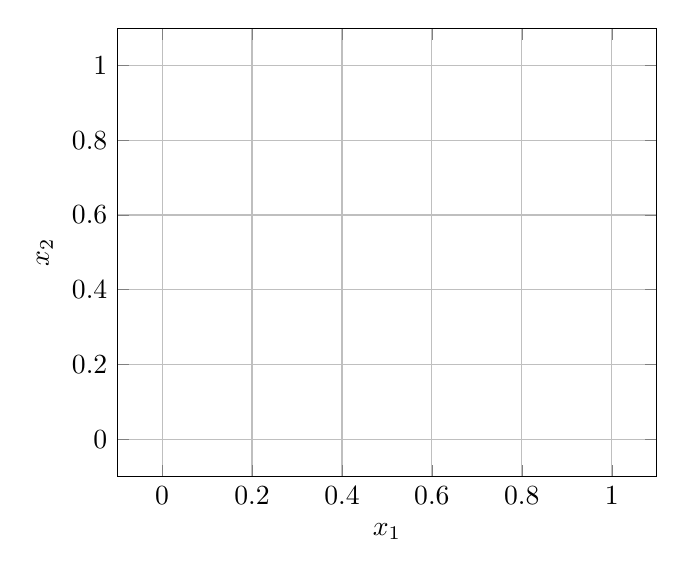
\begin{tikzpicture}
\begin{axis}[
	grid=major,
	samples=\samples*3,
	xlabel=$x_1$,
    ylabel=$x_2$,
    zlabel=$fitness$
]

\addplot3[surf, unbounded coords=jump]
{
	(x-1)^3 + (y-2) <0  &&
	(x-1)^3 - (y-2) <0  &&
	-x<0 ?
	-x: NaN
};

\end{axis}
\end{tikzpicture}
\end{center}


\[
	f(x) = -x_1 \qquad g(x) = \begin{cases}
		g_1(x) = (x_1-1)^3 + (x_2-2) \leq 0\\
		g_2(x) = (x_1-1)^3 - (x_2-2) \leq 0\\
		g_3(x) = -x_1\leq 0\\
	\end{cases}
\]

Calcolo i gradienti:

\[
	\nabla f = \begin{bmatrix}
	-1\\
	0
	\end{bmatrix}
	\quad
	\nabla g_1 = \begin{bmatrix}
	-3(x_1-1)^2\\
	1
	\end{bmatrix}
	\quad
	\nabla g_2 = \begin{bmatrix}
	3(x_1-1)^2\\
	1-
	\end{bmatrix}
	\quad
	\nabla g_3 = \begin{bmatrix}
	-1\\
	0
	\end{bmatrix}
\]

Realizzo il sistema delle condizioni:

\[
	\begin{cases}
		-1 + \mu_1 3(x_1 -1)^2 + \mu_2 3(x_1-1)^2 + \mu_3(-1) = 0\\
		0 + \mu_1 1 + \mu_2 (-1) + \mu_3 0 = 0 \\
		\mu_1 [(x_1 - 1)^3 + (x_2-2)] = 0 \\
		\mu_2 [(x_1 - 1)^3 - (x_2-2)] = 0 \\
		\mu_3 (-x_1)
	\end{cases}
	\Rightarrow
	\begin{cases}
		\mu_3 = 0\\
		\mu_3 = -1
	\end{cases}
\]

Il sistema preso in analisi è impossibile, per cui non ha \textbf{punti candidati}.

Troviamo, tramite l'analisi dei gradienti indipendenti, dei punti regolari.

\end{document}